\subsection{Calibración}\label{calibracion}

%\subsection{Calibración para secuencias reales}

%\label{seccion_calibracion_secuencias_reales}

%%%%%%%%%%%%REFERENCIAS%%%%%%%%%%%%%%%%%
% LIC DARIO SANTOS, HOSPITAL DE CLÍNICAS

%Se ha podido tener acceso a secuencias de video de análisis del movimiento de la marcha que se han realizado en el Hospital de Clínicas. Dichas secuencias han sido obtenidas por un grupo de médicos e investigadores con el objetivo de analizar el movimiento de pacientes en el ámbito terapéutico o con un objetivo esencialmente de investigación desde el punto de vista de la biomecánica.

%DEBERÍA ACLARARSE QUE ESTO SE HACIA ANTES, CREO QUE TIPO POR 2009 Y AHORA USAN VICON.
%\vspace{-0.3cm}
%\begin{figure}[ht!]
%\centering
%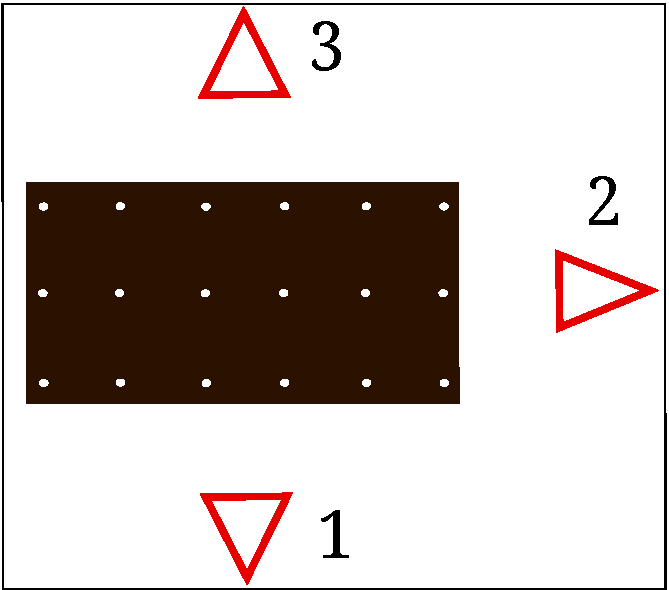
\includegraphics[scale=0.5]{img/calibracion/lab_real.pdf}
%\vspace{-0.3cm}
%\caption{Laboratorio del Hospital de Clínicas.}
%\label{fig: lab_real}
%\end{figure}


%La metodología utilizada consiste en el uso de tres cámaras de video convencionales de 25 fps y resolución  720 x 576 píxeles. Dichas cámaras se disponen como se muestra en la Figura \ref{fig: lab_real}, alrededor de una alfombra o cinta sobre la que se le pide al paciente que camine.\\



%La persona que se desea evaluar debe tener colocados marcadores, fundamentalmente en las articulaciones del cuerpo, y debe desplazarse sobre la alfombra dispuesta para esto. En la Figura \ref{fig: persona con marcadores}, se observa a un individuo caminando con los marcadores colocados.

%\vspace{-0.2cm}
%\begin{figure}[ht!]		
        %\subfloat[Persona con marcadores]{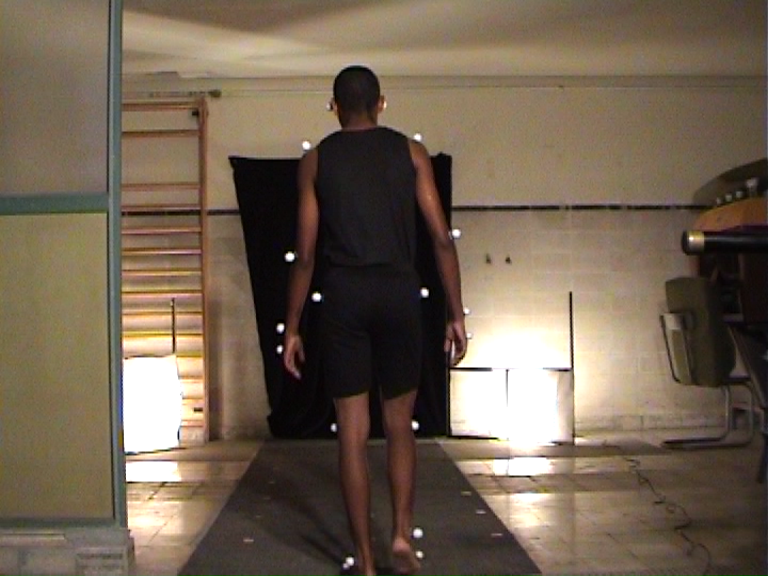
\includegraphics[scale=0.28]{img/calibracion/captura_real.png}\label{fig: persona con marcadores}}
%        \hspace{0.1cm}
        %\subfloat[Objeto de calibración]{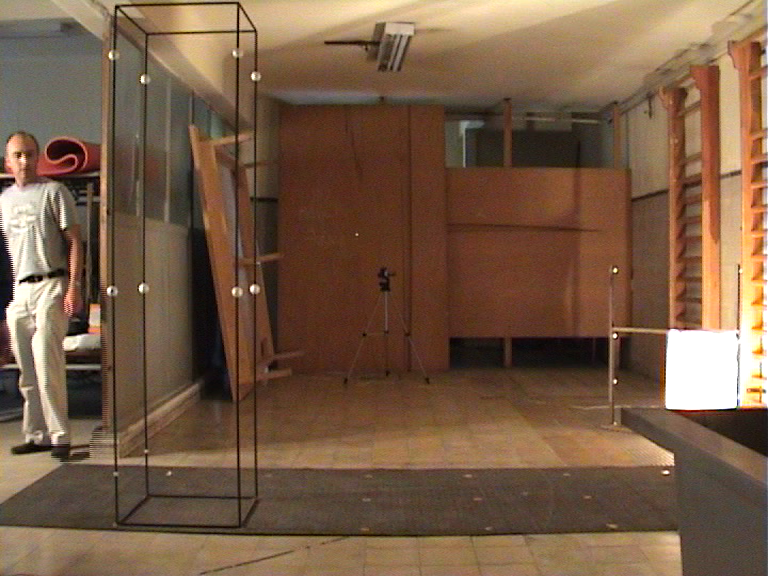
\includegraphics[trim = 20mm 0mm 40mm 0mm, clip, scale=0.28]{img/calibracion/calibrador.png}\label{fig: calibrador}}
%  \caption{Captura de secuencia real}
      \label{fig: captura real}
%\end{figure}

%Antes de la captura del movimiento se emite una señal acústica con la cual se sincronizan las tres vistas una vez obtenidos los videos. El software con el cual este grupo de médicos ha analizado el movimiento es el \textit{Dvideow}.            
 %%%%%%%%%%%%%%%%%%(REFERENCIAR)%%%%%%%%%%%%%%%%%%%%%%%%%%%%%%. 
% Dicho software realiza la detección, seguimiento y reconstrucción de los marcadores. Por otro lado, no se ha podido tener acceso a este software por lo cual tampoco se pudo evaluar su desempeño y compararlo con el desarrollado en este proyecto.\\

%El método que utilizaron para calibrar las cámaras requiere de un objeto de calibración como el que se muestra en la Figura \ref{fig: calibrador}, al que se le llama \textit{fantoma}. Este objeto se compone de marcadores colocados sobre una estructura cuyas dimensiones son conocidas. Dicho objeto se lo coloca en posiciones determinadas que se encuentran marcadas sobre la alfombra, ver Figura \ref{fig: calibrador}. De esta manera se obtiene un mayor número de puntos ubicados en el volumen de trabajo.\\


%Los videos proporcionados por los especialistas del Hospital de Clínicas incluyen tanto las secuencias de marcha de diferentes individuos como el proceso con el que se calibran las cámaras del laboratorio. A partir de dichos videos se desarrolló un algoritmo tal que permite extraer las matrices de proyección de cada una de las cámaras. Tomando un cuadro del video en el que se encuentre el \textit{fantoma} en una de las posiciones, el algoritmo implementado requiere que cada marcador del \textit{fantoma}, en cada una de las vistas, sea seleccionado manualmente, y en un orden tal que permita establecerse una correspondencia entre las proyecciones de un mismo marcador en las tres vistas. En la Figura \ref{fig: vistas_calibrador} se muestra a uno de los marcadores seleccionado en cada una de las vistas.
%\vspace{-0.53cm}
%\begin{figure}[ht!]
%        \hspace{-1cm}
        %\subfloat[Vista cámara 1]{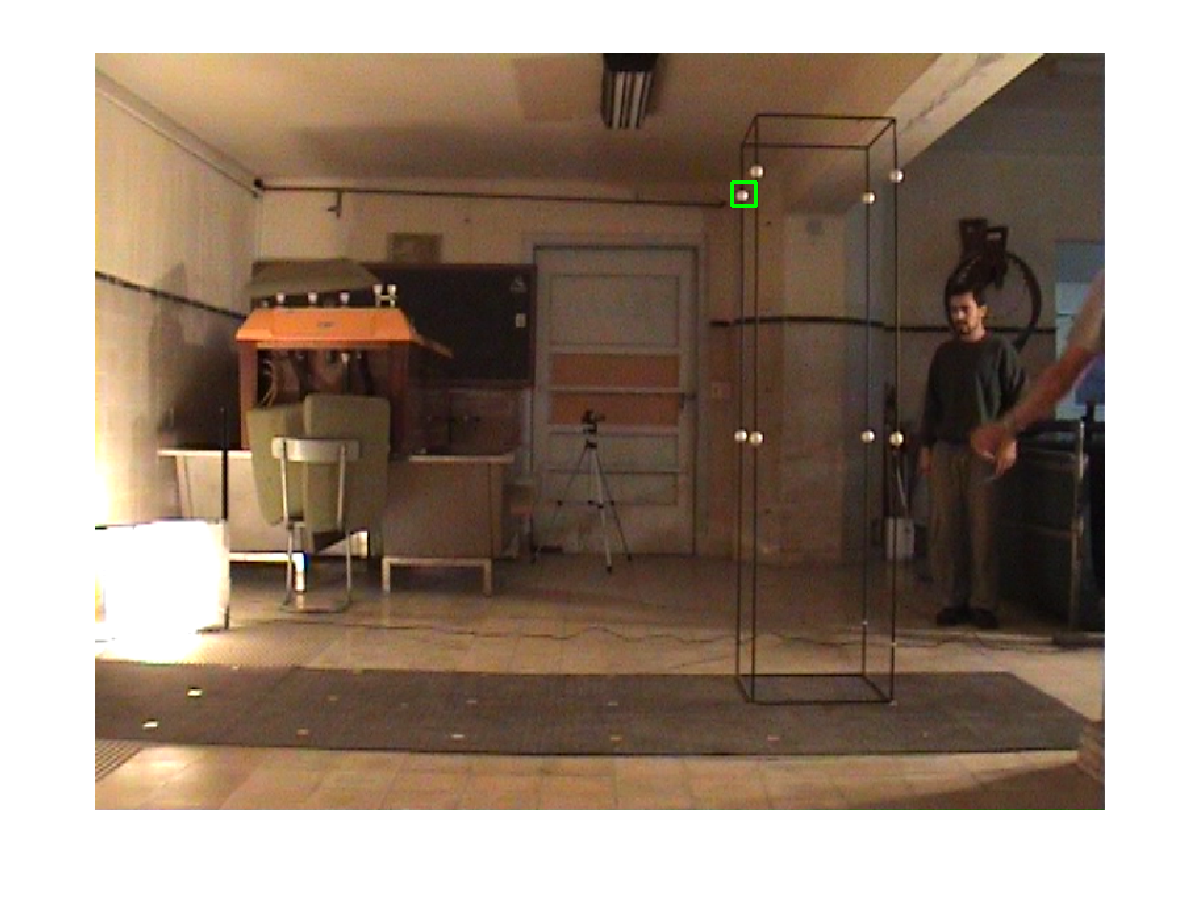
\includegraphics[trim = 59mm 0mm 41mm 0mm, clip,scale=0.45]{img/calibracion/calibrador_cam1.png}}
%                \hspace{1mm}
       % \subfloat[Vista cámara 2]{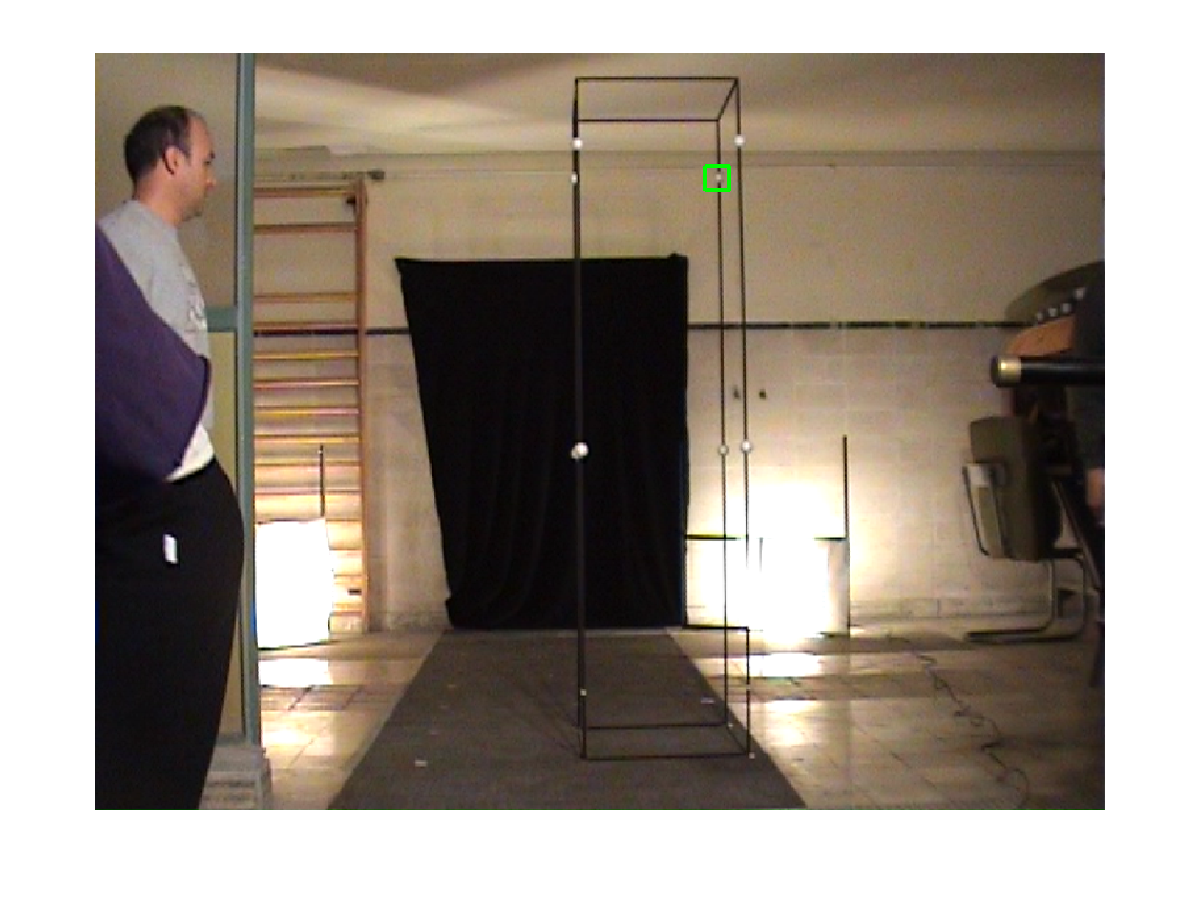
\includegraphics[trim = 50mm 0mm 50mm 0mm, clip,scale=0.45]{img/calibracion/calibrador_cam2.png}}     	
%  \hspace{1mm}
        %\subfloat[Vista cámara 3]{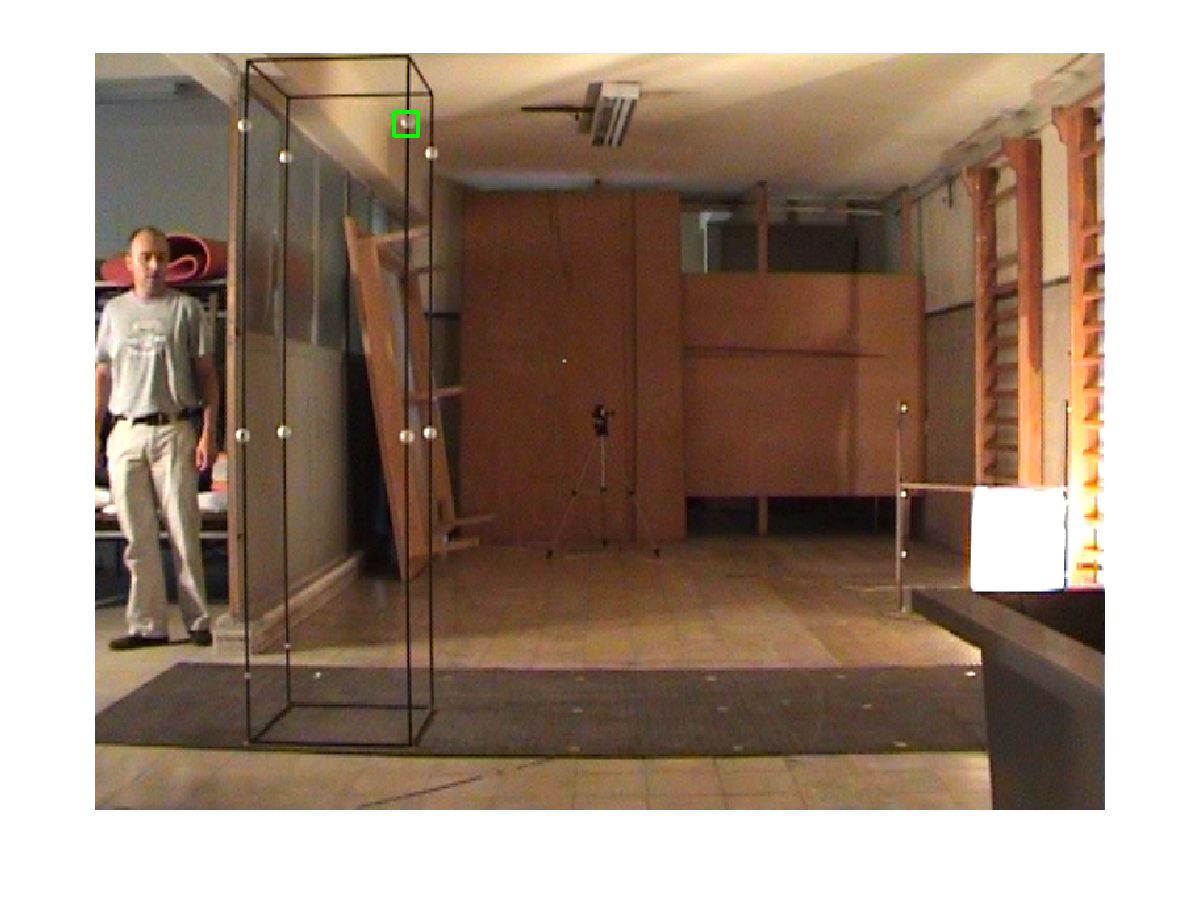
\includegraphics[trim = 32mm 0mm 68mm 0mm, clip,scale=0.45]{img/calibracion/calibrador_cam3.png}}
      
%      \caption{Uno de los marcadores de calibrador seleccionado en cada una de las cámaras}
%      \label{fig: vistas_calibrador}      
%\end{figure}


%Por otra parte la posición de los marcadores en el espacio 3D es conocida ya que se saben las medidas del \textit{fantoma}, ver Figura \ref{fig: medidas_calibrador}. Dichas posiciones pueden ser referidas un punto que puede elegirse arbitrariamente, así como los ejes de coordenadas $(x,y,z)$.

%\vspace{-0.53cm}
%\begin{figure}[ht!]
%        \centering
     %{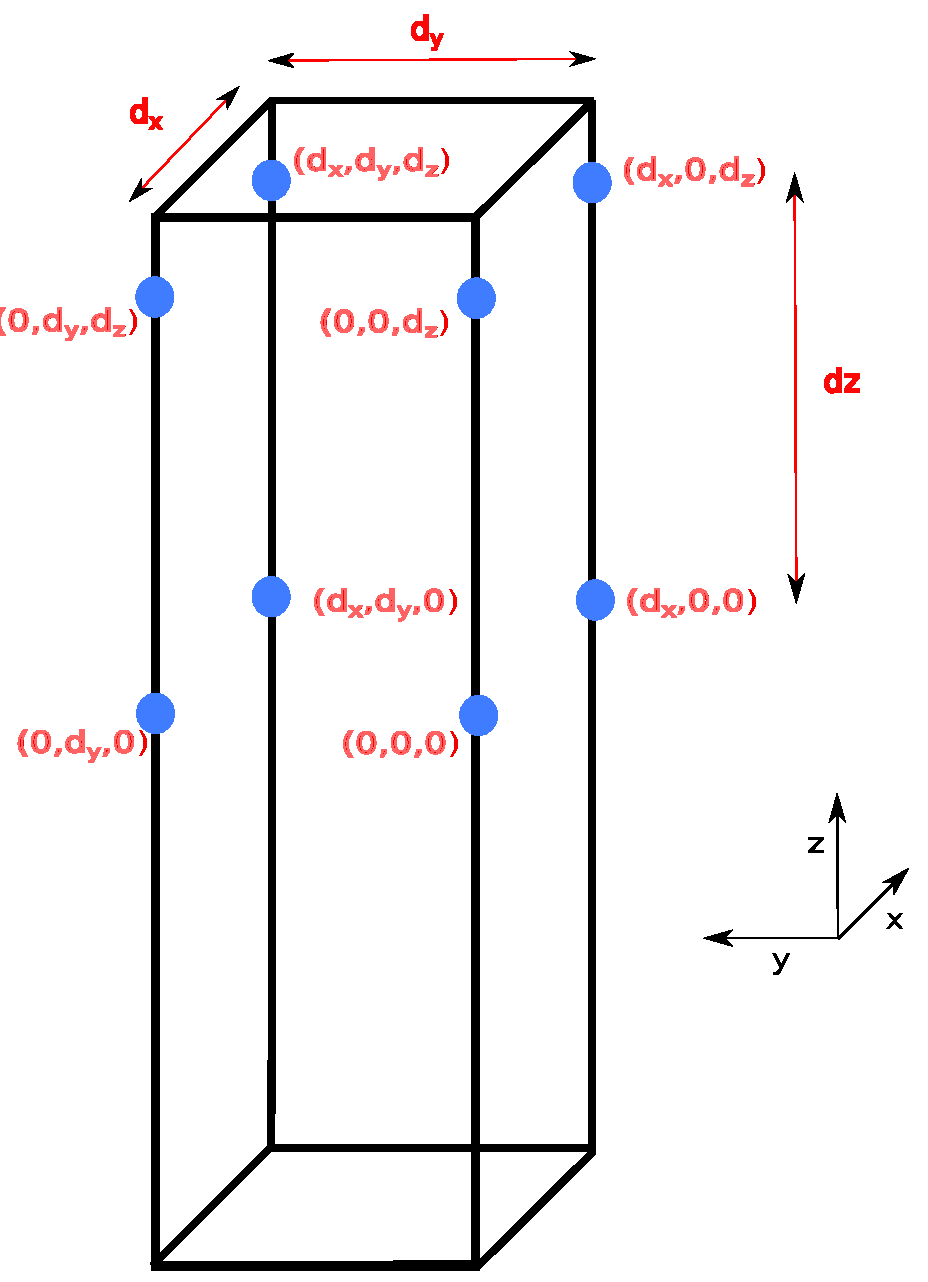
\includegraphics[scale=0.38]{img/calibracion/medidas_calibrador.pdf}}    
%     \caption{Coordenadas de los marcadores del \textit{fantoma}}
%      \label{fig: medidas_calibrador}     
%\end{figure}

%  De esta forma se tiene asociadas las coordenadas 3D de los marcadores en el espacio con sus correspondientes coordenadas 2D en píxeles en cada una de las cámaras, $\mathbf{X_i} \leftrightarrow  \mathbf{x_i}$. Si se tiene una cantidad suficiente de puntos, entonces las matrices de proyección $P$ pueden ser estimadas tal que $\mathbf{x_i}=P\mathbf{X_i}$. Para esto se utiliza el algoritmo \textit{Direct Linear Transformation (DLT)}.\\
   
% Según lo demostrado en \cite{hartley}, para cada asociación de puntos $\mathbf{X_i} \leftrightarrow \mathbf{x_i}$ se cumple que :
   
%   \[
%   \begin{pmatrix}
%   0^T & -w_iX_i^T & y_iX_i^T \\
%   w_iX_i^T & 0^T & -x_iX_i^T
%   \end{pmatrix}
%   \begin{pmatrix}
%    P^1 \\
%    P^2 \\
%    P^3
%   \end{pmatrix}
%   = 0   
%      \]
   
   
% \hspace{-0.6cm}siendo $P^{iT}$ las columnas $i$-ésimas de $P$ y $\mathbf{x_i}$ de coordenadas homogéneas $(x_i,y_i,w_i)$. Dicha matriz se obtiene resolviendo un conjunto de ecuaciones del tipo $Ap=0$.  Dado que por cada punto se tiene dos ecuaciones y que la matriz $P$ tiene doce entradas y once grados de libertad, ignorando el factor de escala, resulta que son necesarios conocer al menos seis correspondencias $X_i \leftrightarrow x_i$.\\
 
%Para anular los efectos de la selección arbitraria del origen y la escala del sistema de coordenadas se aplica una normalización tanto a los puntos imagen 2D como a los 3D, logrando de esta manera mejorar los resultados finales. Para los puntos 2D de cada vista se traslada el origen de coordenadas de dicha vista al centroide de los puntos y se aplica un escalado tal que la distancia promedio de los puntos al origen sea $\sqrt{2}$. Para los puntos 3D el mismo procedimiento excepto que el escalado que se aplica es tal que la distancia promedio al origen es $\sqrt{3}$. De esta manera se tiene dos matrices que realizan esta transformación, la matriz $T_{3D}$ tal que $\tilde{X_i} = T_{3D}^{}X_i$ para los puntos en el espacio, siendo $\tilde{X_i}$ los puntos normalizados. Análogamente para los 2D imagen se tiene la matriz $T_{2D}^{}$ tal que $\tilde{x_i} = T_{2D}^{}x_i$. \\
 
% Dado que las coordenadas de los puntos 2D están afectadas por el ruido y que se tienen más de seis correspondencias $X_i \leftrightarrow x_i$, no existe una solución exacta a las ecuaciones $Ap=0$. Por lo tanto la solución se obtiene minimizando un error, en este caso se busca $p$ tal que minimice $||Ap||$. Para esto se utiliza la descomposición en valores singulares (SVD), donde se obtiene del vector singular asociado al menor valor singular. De esta manera se obtiene la matriz de proyección $\tilde{P}$. Por último debe descomponerse la normalización, por lo tanto la matriz de proyección $P$ queda $P = T_{2D}^{-1} \tilde{P} T_{3D}^{}$.
 
%\subsection{Calibración simulada en \emph{Blender}}
 Para establecer una metodología de calibración válida para la configuración de cámaras con las que se diseñó el entorno virtual descrito en la sección \ref{section_base_de_datos}, se probaron distintas implementaciones existentes, evaluando dos toolbox elaborados en \emph{Matlab}. La metodología de calibración fue simulada en \emph{Blender} mediante \textit{scripts} \emph{Python} y las imágenes resultantes procesadas con dichos toolbox. La descripción de la metodología y las simulaciones se detalla en \cite{proyecto_biomecanica}.\
 
 Uno de los toolbox utilizados es el \textit{Automatic Multi-Camera Calibration Toolbox (amcctoolbox)} \cite{amcctoolbox}, el cual utiliza como objeto de calibración un damero. Este método, con resultados de buena precisión \cite{zhang_libro}, puede no ser suficientemente flexible para un sistema de muchas cámaras ya que, entre otras cosas, es necesaria la intervención manual en algunos casos.\
 
El otro toolbox utilizado es el \textit{Multi-Camera Self-Calibration Toolbox} \cite{toolbox_led}. Este método consiste en capturar el movimiento de una fuente puntual de luz que recorra el volumen de trabajo. Para cada cuadro se tiene un punto 3D en el espacio en una posición distinta y en cada una de las cámaras su correspondiente proyección.
 El error de re-proyección promedio obtenido es menor a 0.13 píxeles para todas las cámaras. Este método plantea una forma simple de calibrar un conjunto de muchas cámaras adecuado para el sistema de 17 cámaras del laboratorio virtual desarrollado en \emph{Blender}.

 
 
%\subsubsection{Automatic Multi-Camera Calibration Toolbox (amcctoolbox) }\cite{amcctoolbox}  


%Esta herramienta automatiza ciertas funciones del toolbox \textit{Camera Calibration Toolbox}, reduciendo la intervención del usuario. Utiliza como objeto de calibración un damero.

%Para la calibración de conjuntos de varias cámaras, el damero debe ser colocado en múltiples ubicaciones y orientaciones cubriendo el mayor volumen de trabajo tal que, en cada una de estas posiciones, el damero pueda ser visto por más de una cámara simultáneamente.

%La calibración del entorno virtual se realiza simulando un damero real. Para cada par de cámaras adyacentes se coloca el damero en algún punto dentro del volumen de trabajo, con una orientación tal que la figura plana del damero sea visible en ambas cámaras. Luego, a partir de dicha posición, se toman capturas del damero cambiando ligeramente la ubicación y orientación del mismo. Para cada par de cámaras adyacentes se consideran entre 15 y 20 posiciones distintas del damero.

%Una vez realizadas las capturas se procesan  las imágenes mediante el toolbox, obteniéndose los parámetros intrínsecos de cada una de las cámaras y la posición relativa de cada uno de los pares de cámaras adyacentes y por lo tanto las posición relativa de todas las cámaras.


%Este método aunque sus resultados tiene buena precision \cite{zhang_libro}, puede no ser suficientemente flexible para un sistema de muchas cámaras, ya que, entre otras cosas, puede ser necesaria la intervención manual en algunos casos.



%\subsubsection{ Multi-Camera Self-Calibration Toolbox } \cite{toolbox_led}
 
 %El procedimiento utilizado en este toolbox consiste en capturar el movimiento de una fuente puntual de luz que recorra el volumen de trabajo. Por lo tanto para cada cuadro se tiene un punto 3D en el espacio en una posición distinta y en cada una de las cámaras su correspondiente proyección si dicho punto es visible desde la cámara. Para esto debe existir un contraste suficiente de la fuente puntual de luz respecto al laboratorio. La fuente de luz puede ser por ejemplo, una lámpara led.
 
%La simulación de este procedimiento se logra creando un punto 3D que toma para cada cuadro, distintas posiciones en forma aleatoria dentro del volumen de trabajo. Para cada cuadro se \textit{renderiza} su posición en las 17 cámaras. En este caso se han tomado 500 posiciones distintas.

% El error de re-proyección promedio obtenido es menor a 0.13 píxeles para todas las cámaras. Este método plantea una forma simple de calibrar un conjunto de muchas cámaras adecuado para el sistema de 17 cámaras del laboratorio virtual desarrollado en \emph{Blender}.

%En la Figura \ref{fig: error reproyeccion} se muestra en azul el promedio y en rojo la desviación estándar del error de re-proyección obtenido para cada una de las cámaras. Sea $X$ un punto 3D en el espacio cuya posición es a priori desconocida y $x$ su correspondiente proyección en un cámara. A partir del resultado de la calibración se obtiene la matriz de proyección $P$ de dicha cámara. A su vez, es posible obtener la estimación del  punto $X$, siendo $ \hat{X}$ dicha estimación. La proyección de $\hat{X}$ sobre la cámara es $\hat{x} = P \hat{X}$. El error de re-proyección de $\hat{X}$ se define como la distancia euclídea $d(x,\hat{x})$ entre los vectores $x$ y $\hat{x}$.\\

%\begin{figure}[ht!]
%\begin{center}
%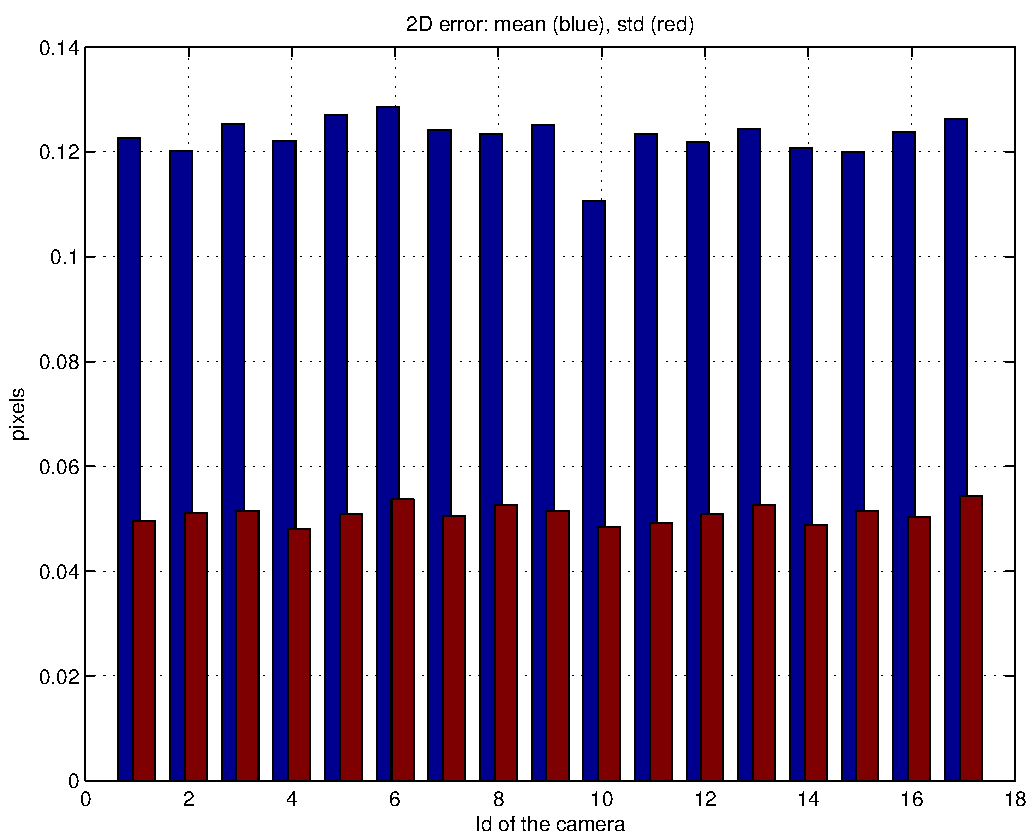
\includegraphics[scale=0.5]{img/calibracion/reprerrors.pdf}
%\end{center}
%\caption{Promedio y desviación estándar del error de re-proyección en todas las cámaras }
%\label{fig: error reproyeccion}
%\end{figure}
  
  
%  Como se observa de la Figura se obtienen errores menores a 0.13 píxeles para todas las cámaras.
  
%\subsubsection{Ajuste del sistema de coordenadas.}

%De los dos toolbox vistos anteriormente se obtuvieron los parámetros intrínsecos y extrínsecos de las cámaras. En el \textit{Multi-Camera Self-Calibration Toolbox} las parámetros extrínsecos de las cámaras son referidos a un sistema de coordenadas desconocido que se establece en el proceso de calibración del toolbox. El origen de coordenadas de ese sistema se ubica en el centroide de todas las posiciones capturadas de la fuente de luz. En el \textit{amcctoolbox} por otra parte, los parámetros extrínsecos de las cámaras son referidos al sistema de coordenadas de la cámara que se definió como el origen del sistema de coordenadas.\\

 %En algunos casos puede desearse que el sistema de coordenadas del espacio 3D sea definido por el usuario. En nuestro caso para poder comparar el resultado de la calibración con el ground truth, el sistema de coordenadas al que están referidos los parámetros de la calibración, debe coincidir con el sistema de coordenadas  definido en el entorno \emph{Blender}.\\

%Una opción para realizar esto, es colocar en el espacio marcadores en posiciones conocidas y capturar imágenes de dichos marcadores en cada cámara. Se asume que de la calibración se obtuvieron las matrices de proyección para cada una de las cámaras referidas a un sistema de coordenadas del espacio, \textit{a priori}, desconocido. Sea entonces, $S_1$ dicho sistema de coordenadas, y $P_i|_{S_1}$ las matrices de proyección referidas a este sistema, siendo $i$ la $i$-ésima cámara. Sea $S_2$ el sistema de coordenadas que se desea establecer como el nuevo sistema de referencia del espacio 3D, y $P_i|_{S_2}$ las matrices de proyección referidas a este sistema, que se deben encontrar.\\

%Si se colocan marcadores en determinadas posiciones del espacio, entonces son conocidas sus coordenadas respecto al sistema $S_2$. Sean $X_j|_{S_2}$ sus coordenadas 3D en el sistema $S_2$, siendo $j$ el $j$-ésimo marcador. Dichos puntos se proyectan en las cámaras en los puntos de coordenadas 2D $x_j^i$. Con dichos puntos y las correspondientes matrices de proyección $P_i|_{S_1}$ es posible conocer las coordenadas de los puntos $X_j$ respecto al sistema $S_1$, esto es, $X_j|_{S_1}$. Con lo cual se tienen las coordenadas de los $j$ marcadores en ambos sistemas de coordenadas. De esta manera es posible inferir la transformación $Tr$ tal que $Tr(X_j|_{S_1}) = X_j|_{S_2}$. Si se aplica el cambio de base a las matrices de proyección se obtiene $Tr(P_i|_{S_2}) = P_i|_{S_1} $. Dicha transformación es una composición de una traslación y una rotación.


%\subsection{Conclusiones}

%En el presente capítulo se han tratado varios métodos de calibración y se ha expuesto porqué dicho proceso es necesario para conocer los parámetros de las cámaras en sistemas de captura. Se ha visto además que de la calibración se obtienen ciertos parámetros que son intrínsecos y otros extrínsecos a las cámaras, basados en el modelo \textit{pinhole} de cámara. Por otra parte se describe cómo obtener los parámetros de calibración a partir de la información proporcionada por el entorno \emph{Blender}, esto último permite conocer el \textit{ground truth} de la calibración para un conjunto de cámaras así como el \textit{ground truth} de la detección de marcadores en las imágenes 2D.\\

%Se implementó un algoritmo que realiza la calibración de cámaras, para la metodología particular utilizada en la captura de movimiento realizada a pacientes en el Hospital de Clínicas. Dicha metodología plantea la utilización de una estructura tridimensional con marcadores ubicados convenientemente. Una característica de este método es que permite abarcar todo el volumen de trabajo. Asimismo el uso de objetos 3D para la calibración ofrece mayor precisión \cite{zhang_libro}. Sin embargo, tiene como desventaja que requiere la intervención del usuario en el proceso de calibración, con lo cual resulta en un metodología poco adecuada para calibrar un sistema de muchas cámaras.\\



%el metodo para el caso real permite abarcar todo el volumen de trabajo, tiene mayor precision pero requiere la interviencion del usuario  por lo que no es adecuado para calibrar un conjunto de muchas camaras.




%Por otra parte se han utilizado dos toolbox elaborados en \emph{Matlab}, para calibrar las cámaras del laboratorio virtual implementado en \emph{Blender}. Para esto se ha simulado en el mismo entorno \emph{Blender} una calibración real utilizando estos toolbox.\\


%El \textit{amcctoolbox}, plantea un método muy utilizado para la calibración de cámaras a través de objetos planos, en nuestro caso un damero, cuyos resultados poseen buena precisión \cite{zhang_libro}. Sin embargo presenta la desventaja de que los parámetros extrínsecos de las cámaras se vinculan en relación a sus adyacentes, por lo que debe definirse a una de las cámaras como el origen del sistema de coordenadas del espacio, respecto a la cual se halla la posición del resto de las cámaras. Por lo tanto el error se acumula incrementándose en aquellas cámaras que están más alejadas de aquella que se define como el origen del sistema. Este toolbox por otra parte, requiere para la calibración de un par cámaras, establecer en forma automática una correspondencia entre la imagen del damero detectado en la cámara izquierda con la imagen capturada por la cámara derecha. Esto en algunos casos no se logra y la correspondencia entre dichas imágenes debe realizarse en forma manual. \\





%Debe considerarse para trabajos futuros, además de los aspectos cualitativos expuestos,  una evaluación de performance de los métodos considerados, teniendo en cuenta las diferencias implicadas en la calibración de un sistema de pocas o muchas cámaras.\\